% !TEX program = xelatex

\documentclass[hidelinks, 12pt, a4paper]{article}

\usepackage{fontspec}
\setmainfont[Ligatures=TeX]{Linux Libertine O}

\usepackage[hidelinks, colorlinks = true, urlcolor = blue]{hyperref}

\usepackage{indentfirst}
\usepackage{graphicx}
\usepackage[left=2cm,right=2cm,top=2cm,bottom=2cm]{geometry}
\usepackage{lipsum}
\usepackage{caption}
\usepackage{subcaption}
\usepackage{dirtytalk}
\usepackage[autostyle]{csquotes}
\usepackage{epigraph}


\begin{document}
\sloppy % this is legendary

\begin{titlepage}

\begin{figure}[h!]
  \begin{center}
    
\includegraphics[width=3cm]{assets/auth.pdf}
    \label{fig:cover_auth_logo}
  \end{center}
\end{figure}

\centering
\Large Αριστοτέλειο Πανεπιστήμιο Θεσσαλονίκης\\
\Large Πολυτεχνική Σχολή\\
%\large Τμήμα Ηλεκτρολόγων Μηχανικών και Μηχανικών Υπολογιστών\\
%\large Τομέας Τηλεπικοινωνιών

\vspace{\fill}

%\LARGE \textbf{Java socket programming} \\
\LARGE \textbf{Δίκτυα Υπολογιστών Ι}

\vspace{\fill}

\Large Θεόδωρος Κατζάλης \\
\Large ΑΕΜ:9282 \\ 
\Large katzalis@auth.gr

\vspace{\fill}
\raggedright

\centering
\vspace{\fill}
\today

\end{titlepage}

%\maketitle


\pagebreak
{
\renewcommand*\contentsname{Περιεχόμενα}
\hypersetup{linkcolor=black}
\tableofcontents
}
\pagebreak

% \section{Lorem}
% \lipsum


\section{Εισαγωγή}

Η συγκεκριμένη εργασία αποσκοπεί στην εξοικείωση εννοιών σχετικά με τα δίκτυα υπολογιστών τόσο σε θεωρητικό όσο και σε πρακτικό επίπεδο. Αυτό εξασφαλίζεται με την δημιουργία δικτυακών εφαρμογών χρησιμοποιώντας την γλώσσα προγραμματισμού \textbf{java} σε συνεργασία με τον server ithaki του μαθήματος με IP 155.207.18.208. Αυτή λοιπόν η συνεργασία αποσκοπεί στην συλλογή δεδομένων επειτα απο συγκεκριμένα request του χρήστη στον server. Αρχικά θα σχολιάσουμε τα αποτελέσματα που πήραμε σε δύο συνόδους, στη συνέχεια θα αναλύσουμε τον πηγαίο κώδικα και στο τέλος αυτού του report θα γίνει μια σύντομη αναφορά σε μηχανισμούς και πρωτόκολλα modem.

\subsection{Statement of originality}

Αξίζει να αναφερθεί ότι η εργασία ξεκίνησε με βάση το seed code της Ιθάκης. Για λόγους πληρότητας και διαφάνειας παραθέτουμε, στο τέλος της αναφοράς, τις πηγές για την επίλυση των προβλημάτων που συναντήσαμε κατά την εκπόνηση της. Τα εργαλεία που χρησιμοποιήθηκαν ήταν ένας text editor και ένας terminal emulator σε Linux περιβάλλον, αποφεύγοντας την χρήση IDE όπως Eclipse! Αυτό μας έδωσε την δυνατότητα να έχουμε μια πιο ολοκληρωμένη επίγνωση της διαδικασίας που πολλές φορές IDE προσπαθούν, για λόγους ευκολίας, να την αποκρύψουν. Ακόμη, για να διευκολυνθεί η διαδικασία του compile, χρησιμοποιήσαμε make για build automation. Για την δημιουργία των διαγραμμάτων, χρησιμοποιήσαμε python και την βιβλιοθήκη matplotlib. Τέλος, το συγκεκριμένο έγγραφο έγινε με την χρήση \LaTeX! 

\section{Session 1}
Σχετικά με τα διαγράμματα του session 1 έχουμε να αναφέρουμε τα εξής:

\subsection{G1}

Για να μπορούμε να καταλάβουμε τις ιδιότητες του χρόνου απόκρισης των echo packets συμπληρώσαμε στα γραφήματα ένα ιστόγραμμα και μια zoom in εκδοχή του διαγράμματος. Θα μπορούσαμε να ισχυριστούμε ότι ο χρόνος απόκρισης ακολουθεί bimodal κατανομή εξαιτίας των δύο κορυφών. Ακόμη βλέποντας την zoom in εκδοχή παρατηρούμε μια ταλάντωση γύρω απο την τιμή 30 milliseconds, στην οποία βρίσκεται και η κορύφωση του ιστογράμματος.

\subsection{G2}

Σχετικά με το ΑRQ παρατηρούμε spikes στο διάγραμμα της απόκρισης του χρόνου. Αυτο είναι αναμενόμενο, διότι σε αυτά τα σημεία είχαμε επαναλαμβανόμενες αποτυχίες λήψης ορθού πακέτου, με αποτέλεσμα να υπάρχει χρονοκαθύστερηση εξαιτίας των επιπρόσθετων NACK πακέτων.

\subsection{G3}

Ωστόσο, αυτά τα spikes δεν εμφανίζονται σε πολύ μεγάλη συχνότητα με αποτέλεσμα η πλειοψηφία των πακέτων να ολοκληρώνουν την διαδικασία λήψης πληροφορίας περίπου σε 50 milliseconds. Έτσι βλέποντας το ιστόγραμμα G3, μπορούμε να ισχυριστούμε ότι ακολουθεί right skewed κατανομή.

\section{Session 2}

Σχετικά με τα διαγράμματα του session 2 έχουμε να αναφέρουμε τα εξής:
\begin{itemize}
    \item Παρατηρούμε ότι μπορούμε να εξάγουμε παρόμοια συμπεράσματα με αυτά του session 1.
\end{itemize}

\section{Ανάλυση πηγαίου κώδικα}

Η \textbf{αναγνώριση της ολοκληρωμένης λήψης echo πακέτου} μπορεί να γίνει με διάφορες προσεγγίσεις. Αξίζει να σημειωθεί ότι στα αρχικά στάδια ανάπτυξης του κώδικα, δεν είχαμε κάποια τεχνική αναγνώρισης και χρησιμοποιούσαμε την ίδια λογική του seed code της Ιθάκης. Δηλαδή ελέγχαμε αν συναντούσαμε τιμή -1 κατά τη ροή λήψης πληροφορίας, το οποίο σηματοδοτούσε οτι η ροή δεν είναι πλέον διαθέσιμη. Στη συνέχεια, παρατηρώντας την μορφή του πακέτου, χρησιμοποιήσαμε ως λέξη κλειδί ολοκλήρωσης το "PSTOP". Συνεπώς για την υλοποίηση αυτού του εντοπισμού, δημιουργήσαμε μια ουρά FIFO η οποία δέχεται διαδοχικά όλα τα σύμβολα του μηνύματος ένα προς ένα. Μόλις συναντήσει το "PSTOP" γίνεται έξοδος της επανάληψης λήψης χαρακτήρων. Φυσικά η συγκεκριμένη αναγνώριση έπρεπε να γίνει προκειμένου να έχει νόημα και η χρονική απόκριση λήψης πακέτων που παρουσιάστηκε στα αρχεία με τα διαγράμματα.

'Οσον αφορά τον τερματισμό της εικόνας, μετατρέπαμε την λαμβανόμενη πληροφορία σε δεκαεξαδική μορφή και ελέγχαμε τον delimiter \verb|0xFFD9|. Στη συνέχεια αποθηκεύαμε το αρχείο σε μορφή jpg.

Σχετικά με το \textbf{GPS} και τα στίγματα, αξίζει να σημειωθεί ότι για λόγους χρηστικότητας, προσπαθήσαμε να αυτοματοποιήσουμε την διαδικασία εντοπισμού στιγμάτων που απέχουν σε σημαντικό βαθμό χρονικά, έτσι ώστε να είναι ευδιάκριτη η διαφορά τους πάνω στην εικόνα. Πιο συγκεκριμένα, συλλέγοντας GPS data points σε \textbf{NMEA format}, κάνοντας parse τα δεδομένα, απομονώσαμε το latitude και το longitude και βρίσκαμε τα σημεία τα οποία διέφεραν στις δύο αυτές τιμές. Φυσικά για να ικανοποιηθεί η παραπάνω απαίτηση, τα σημεία αυτά βλέποντας στη συνέχεια και το χρονικό τους αποτύπωμα, απείχαν τουλάχιστον 4 δευτερόλεπτα μεταξύ τους.

Αρκετά σημαντική λεπτομέρεια στην διαδικασία αποσύνθεσης του NMEA format ήταν η μορφή του \textbf{GPS request code}. Απαιτείται να εισάγεται πρώτα το γεωγραφικό πλάτος και στη συνέχεια το γεωγραφικό μήκος όταν συγχωνεύουμε τις συμβολοσειρές για να δημιουργήσουμε το GPS code, το οποίο είναι ανάποδο με την σειρά την οποία έρχονται τα δεδομένα ως NMEA format! Ακόμη έπρεπε να μετατρέψουμε σε δευτερόλεπτα το δεκαδικό κομμάτι της πληροφορίας των λεπτών που λαμβάναμε, πολλαπλασιάζοντας το με 0,6.

Η διαδικασία του \textbf{ARQ} είχε αρχικά παρόμοια απαίτηση απομόνωσης της ωφέλιμης πληροφορίας με το GPS. Πιο συγκεκριμένα παίρνοντας τα δεδομένα, απομονώσαμε το FCS και την κρυπτογραφημένη συμβολοσειρά. Μετατρέψαμε την συμβολοσειρά σε έναν πίνακα απο χαρακτήρες και στη συνέχεια με διαδοχικές πράξεις XOR υπολογίζαμε αν τελικά η λήψη του πακέτου ήταν ορθή συγκρίνοντας το αποτέλεσμα του XOR με το FCS. Διαφορετικά επαναλαμβάναμε την διαδικασία μέχρι το FCS να ισούται με την κωδικοποιημένη τιμή της ακολουθίας.

Μια λίστα με τις αναφορές που χρησιμοποιήθηκαν κατά την εκπόνηση της εργασίας είναι η ακόλουθη:

\begin{itemize}
    \item Μια γρήγορη ανακεφαλαίωση της γλώσσας προγραμματισμού java \cite{derek}
    \item Πως να μετατρέψεις ακέραιους σε byte array; \cite{int2byte}
    \item Πως να αποθηκεύσεις byte array σε αρχείο; \cite{javafile}
    \item Μετατροπη byte σε hexadecimal \cite{programizhex}
    \item Αποσύνθεση συμβολοσειράς \cite{stackparsestring}
    \item Ημερομηνία και ώρα \cite{timeAndDate}
    \item XOR array \cite{xor}
    \item Java API \cite{javaDocs}
    \item Java Best Practices \cite{javaPractice}
\end{itemize}

Επίσης να σημειώσουμε ότι προσπαθήσαμε ως επι το πλείστον να κάνουμε καλή διαχείριση errors και \textbf{try, catch} blocks προκειμένου να εντοπίζουμε γρήγορα προβλήματα. Για debugging λόγους χρησιμοποιούσαμε print statements σε συνεργασία με command line tools όπως jdb.

\subsection{User Interface}

Φυσικά για αισθητικούς λόγους, προτιμήσαμε κατά την έναρξη της εφαρμογής, να τυπώνουμε το παρακάτω κείμενο (ASCII art)!

\begin{figure}[h!]
\centering
	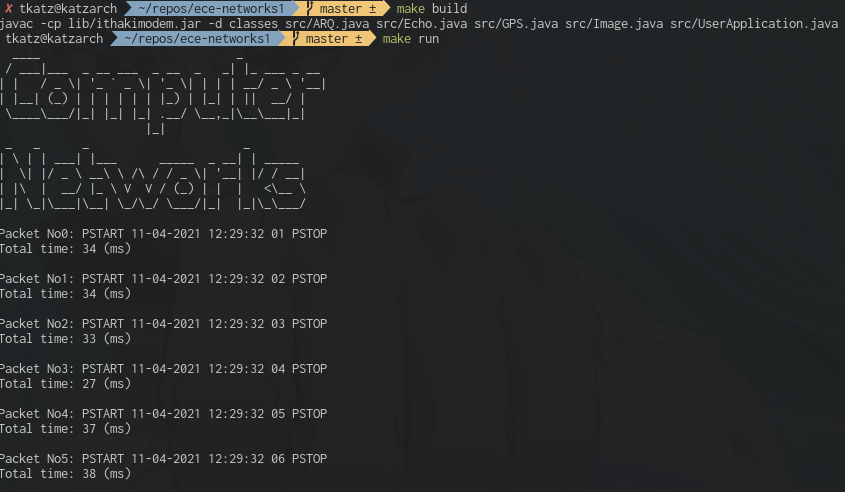
\includegraphics[height=.3\textheight, width=.8\textwidth]{assets/ui_welcome.png}
	\caption{Computer Networks \\ Welcome screen!} 
\end{figure}

Στη συνέχεια ακολουθεί μια σύντομη βιβλιογραφική αναφορά σε μηχανισμούς και πρωτόκολλα modem.

% \begin{figure}
%      \begin{subfigure}[b]{.5\textwidth}
%          \centering
%          \includegraphics[width=\textwidth]{assets/ui.png}
%          \caption{$y=3sinx$}
%      \end{subfigure}
%      \hfill
%      \begin{subfigure}[b]{.5\textwidth}
%          \centering
%          \includegraphics[width=\textwidth]{assets/ui.png}
%          \caption{$y=5/x$}
%      \end{subfigure}
%         \caption{Three simple graphs}
%         \label{fig:three graphs}
% \end{figure}

\pagebreak
\section{Modem}

Η αγγλική λέξη Modem προέρχεται απο την σύνθεση των λέξεων \textbf{MODulation} και \textbf{DEmodulation}. Το πρώτο υποδεικνύει την διαμόρφωση του ψηφιακού σήματος σε αναλογικό και το δεύτερο την αποδιαμόρφωση, η οποία είναι η αντίστροφη διαδικασία, δηλαδή την μετατροπή απο αναλογικό σε ψηφιακό. Η διαμόρφωση είναι μια απο τις βασικές έννοιες των τηλεπικοινωνίων και ο ρόλος της είναι ο μετασχηματισμός της πληροφορίας σε μια μορφή κατάλληλη η οποία μπορεί να προσαρμοστεί και να ανταπεξέλθει στις ιδιότητες του μέσου επικοινωνίας (θόρυβος) σε συνδυασμό με τις απαιτήσεις (για παράδειγμα πολυπλεξία). To modem λοιπόν αποτελεί δομικό στοιχείο σε ένα δίκτυο υπολογιστών και θα δούμε το γιατί αναλύοντας την δομή και τις εφαρμογές του. Πολλές φορές συγχέονται οι έννοιες \textbf{router} και \textbf{modem}, διότι συνήθως, σε οικιακό επίπεδο, έχουμε στα χέρια μας συσκευές οι οποίες υλοποιούν και τις δύο λειτουργίες. Ωστόσο το router είναι μια ψηφιακή συσκευή η οποία είναι υπεύθυνη για την ασύρματη και την ενσύρματη μετάδοση της ψηφιακής πληροφορίας στο τοπικό δίκτυο μέσω Wifi και Ethernet. Αποτελεί δηλαδή μέσο διάδοσης πληροφορίας η οποία προήλθε σε αυτόν τον τοπικό κόμβο μέσω της σύνθετης υποδομής των δικτύων και μεταφράστηκε με την βοήθεια του modem \cite{modem}.

\begin{figure}[h!]
\centering
	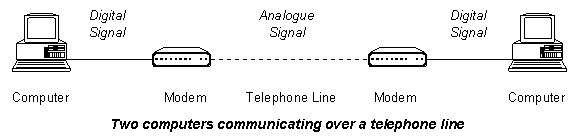
\includegraphics[keepaspectratio, width=.8\textwidth]{assets/modem2.png}
    \caption{source: https://ictsmart.tripod.com/ict4/online/artmoin.htm}
\end{figure}

\subsection{Ιστορική αναδρομή}
Τις εποχές όπου δεν είχε κάθε σπίτι τουλάχιστον απο έναν προσωπικό υπολογιστή, οι τηλεφωνικές γραμμές ήταν η βασικότερη υποδομή επικοινωνίας με σκοπό την μετάδοση των αναλογικών σημάτων που προέκυπταν απο transducers και τις φωνές των ανθρώπων. Αυτό είναι το λεγόμενο Public Switched Telephone Network (PSTN). Τα modems που χρησιμοποιούν την συγκεκριμένη υποδομή ονομάζονται \textbf{"voicebands"} εξαιτίας του στενού εύρους ζώνης της ανθρώπινης φωνής. 

Σε αυτήν την κατηγορία, εκμετάλλευσης του χαλκού του PSTN, ανήκουν επίσης τα λεγόμενα dial-up και DSL (Digital Subscriber Line) modems. Κοινό τους χαρακτηριστικό ήταν η χρήση του τηλεφωνικού δικτύου. Ωστόσο το πρώτο σε αντίθεση με το δεύτερο δεν επέτρεπε την ταυτόχρονη χρήση τηλεφώνου και περιήγησης στο διαδίκτυο. Τα dial-up modems χρησιμοποιούσαν ακριβώς τις ίδιες γραμμές μετάδοσης πληροφορίας στις ίδιες συχνότητες για δύο διαφορετικούς σκοπούς, με αποτέλεσμα οποιαδήποτε χρήση τηλεφώνου, την στιγμή μεταφοράς ψηφιακών δεδομένων, να προσθέτει θόρυβο στην επικοινωνία. Τα DSL ωστόσο δεν έχουν το ίδιο μειονέκτημα. Τα καλώδια χαλκού των τηλεφωνικών γραμμών είναι ικανά να μεταδώσουν πληροφορία μεγαλύτερων συχνοτήτων της ανθρώπινης φωνής. Οπότε το DSL εκμεταλλεύεται ακριβώς αυτο το capacity και η μετάδοση πληροφορίας με σκοπό την επικοινωνία υπολογιστών γίνεται σε διαφορετική υψηλότερη ζώνη συχνοτήτων απο αυτή του τηλεφώνου \cite{modemBritanica}.

Απο την άλλη πλευρά υπάρχουν και τα \textbf{cable modems}. Η υποδομή τους βασίζεται σε fibre-coaxial κανάλια τα οποία αποσκοπούν στην μετάδοση τηλεοπτικών σημάτων με υψηλό εύρος ζώνης. Συνήθως το τηλεοπτικό σύστημα αποτελούσε ενδιάμεσο κομμάτι μεταξύ της σύνδεσης ενός modem με το υπόλοιπο διαδίκτυο (Internet), δηλαδή με την υποδομή των Internet Service Providers. Μάλιστα μιας και αυτό το δίκτυο ταυτόχρονα χρησιμοποιούνταν και για τηλεοπτικά σήματα, οι συχνότητες θα έπρεπε να επιλεχθούν κατάλληλα για να αποφευχθούν παρεμβολές.  

Ειδική κατηγορία των DSL αποτελούν τα asynchronous DSL (ADSL). Χαρακτηριστικό τους είναι η ασυμμετρία στην ταχύτητα μετάδοσης πληροφορίας ανάμεσα στο upload και το download, με το δεύτερο να υπερέχει σημαντικά σε σχέση με το πρώτο. Ο λόγος αυτής της ασυμμετρίας είναι σχεδιαστική επιλογή, διαχειρίζοντας κατάλληλα το εύρος ζώνης, εξαιτίας της συνηθισμένης απαίτησης λήψης πληροφορίας σε μεγαλύτερο όγκο σε σχέση με το ανέβασμα. 

Η ανάγκη για υψηλότερους ρυθμούς μετάδοσης πληροφορίας σε συνδυασμό με την εμφάνιση των οπτικών ινών, οδήγησε στο \textbf{VDSL} (very high bit rate DSL). 'Ενα απο τα βασικά μειονέκτηματα του DSL είναι η εξάρτηση της ταχύτητας απο το μήκος των καλωδίων. Προκειμένου να αντιμετωπιστεί αυτό το πρόβλημα, η παρεμβολή \textbf{οπτικών ινών} στο δίκτυο \textbf{χάλκινων αγωγών}, μικραίνει το κομμάτι της χάλκινης διαδρομής, επιτυγχάνοντας έτσι υψηλότερους ρυθμούς μετάδοσης πληροφορίας. Φυσικά η εγκατάσταση οπτικής ίνας καθόλης της διαδρομής της επικοινωνίας αποτελεί μια σύγχρονη προσέγγιση με πολύ υψηλές ταχύτητες (Fiber to the home). Ωστόσο προσπαθούμε σε γενικές γραμμές να χρησιμοποιούμε ότι ήδη υπάρχει (χάλκινους αγωγούς τηλεφωνικού δικτύου). Οπότε το VDSL θα μπορούσαμε να το χαρακτηρίσουμε μια υβριδική επιλογή μεταξύ οπτική ίνας και χαλκού. Για να επιτευχθεί κάτι τέτοιο, οι τηλεφωνικές εταιρείες προσπαθούν να αντικαταστήσουν τμήματα χαλκού με οπτικές ίνες μέχρι το κουτί παρόχου (Fiber to the Curb). Στη συνέχεια η πληροφορία διακλαδίζεται στους πελάτες με μικρές πλέον χάλκινες διαδρομές μέχρι να φτάσει στον εκάστοτε τελικό κόμβο \cite{vdsl}.

\begin{figure}[h!]
\centering
	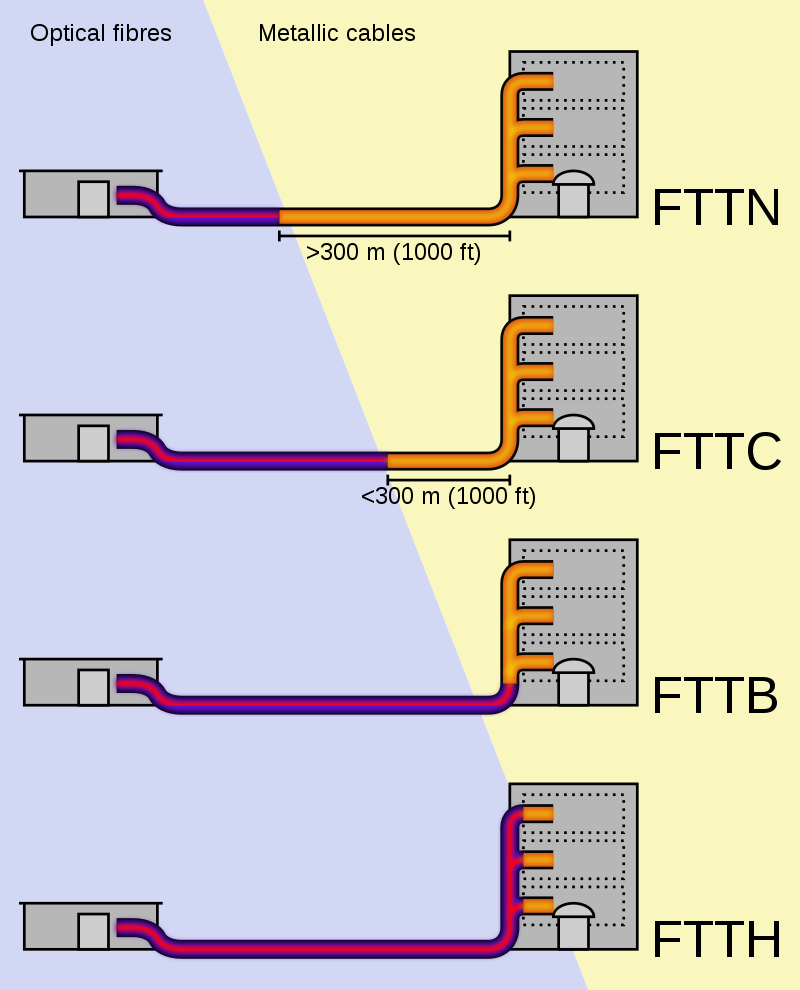
\includegraphics[keepaspectratio, width=.5\textwidth]{assets/fftx.png}
    \caption{Fiber to the x \\ \href{https://en.wikipedia.org/wiki/Fiber_to_the_x}{source}}
\end{figure}

\subsection{Πρωτόκολλα modem}

\subsubsection{Διαμόρφωση}

Μια απο τις μεθόδους διαμόρφωσης της ψηφιακής πληροφορίας σε αναλογική είναι η διαμόρφωση μετατόπισης συχνότητας (\textbf{FSK}). Πιο συγκεκριμένα ας υποθέσουμε ένα πολύ απλό παράδειγμα όπου ο στόχος είναι να μεταδώσουμε το γράμμα 'a' μεταξύ δύο υπολογιστών. Σύμφωνα με τον κώδικα ASCII η bit αναπαράσταση του 'a' είναι 01100001. Ορίζοντας δύο σήματα διαφορετικών συχνοτήτων (δύο τόνοι) και αντιστοιχίζοντας τα με τις λογικές τιμές 1 και 0, έχουμε πλέον διαμορφώσει την ψηφιακή πληροφορία σε αναλογική. Παρόμοιες τεχνικές διαμόρφωσης είναι και η διαμόρφωση μετατόπισης φάσης (\textbf{PSK}), στην οποία πλέον η διαφορά έγκειται στην φάση μεταξύ των σημάτων. Πολύ γνωστή τεχνική είναι και το \textbf{QAM}, του οποίου το πλεονέκτημα είναι  να εμπεριέχεται μεγάλη ποσότητα πληροφορίας σε στενό εύρος ζώνης \cite{fsk}.

\begin{figure}[h!]
\centering
	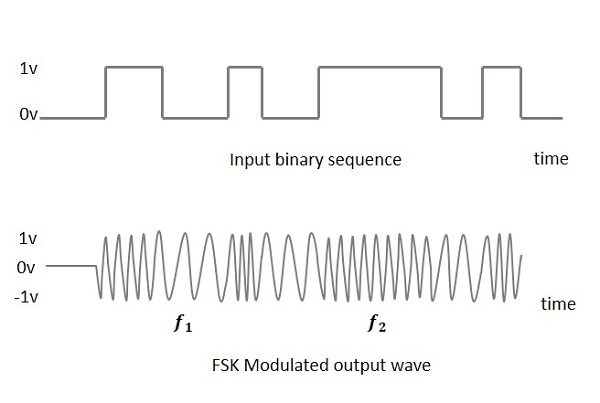
\includegraphics[keepaspectratio, width=.5\textwidth]{assets/fsk.jpg}
    \caption{\href{https://www.tutorialspoint.com/digital_communication/digital_communication_frequency_shift_keying.htm}{source}}
\end{figure}

\subsubsection{Ανίχνευση και διόρθωση σφάλματος}

Ευρέως διαδεδομένη τεχνική ανίχνευσης σφαλμάτων σε μια επικοινωνία είναι τα λεγόμενα checksums και το Cyclic Redudancy Check (CRC). Η κεντρική ιδέα είναι η προσθήκη ενός check value στο τέλος του μηνύματος το οποίο υπολογίζεται αλγοριθμικά με βάση την αλληλουχία bits που πρόκειται να σταλθούν. Στη συνέχεια αυτή η τιμή, απο την πλευρά του δέκτη, υπολογίζεται ξανά με βάση το λαμβανόμενο πακέτο και συγκρίνεται με το αρχικό check value. Αν οι τιμές αυτές είναι διαφορετικές σημαίνει ότι υπάρχει σφάλμα στο μήνυμα μετάδοσης, με αποτέλεσμα να ζητείται επαναποστολή του μηνύματος ή να εφαρμόζεται κάποια τεχνική διόρθωσης του.

Οι αλγόριθμοι που βασίζονται στον υπολογισμό αυτού του check value υλοποιούνται σε hardware ή σε software πραγματοποιώντας πολυωνυμική διαίρεση. Πιο συγκεκριμένα θα μπορούσαμε να αναφέρουμε το εξής: Έστω ότι θέλουμε να μεταδώσουμε το ακόλουθο bit stream 1101011011. Οι ακολουθίες bits σε CRC μπορούν να αντιμετωπιστούν ως συντελεστές πολυωνύμων. 'Ενα πολυώνυμο της μορφής $x^4 + x + 1$ αναπαριστάται σε 10011. Έχουμε δηλαδή ένα πολυώνυμο \textbf{4ης τάξης}. Στη συνέχεια προσθέτουμε 4 μηδενικά, όσα δηλαδή και η τάξη του πολυωνύμου, στο αρχικό bit stream και έχουμε 1101011011\textbf{0000}. Τέλος πραγματοποιούμε διαίρεση μεταξύ του 1101011011\textbf{0000} και 10011. Το υπόλοιπο της διαίρεσης είναι το check value (1110). Φυσικά η επιλογή της πολυωνυμικής συνάρτησης που θα πραγματοποιηθεί η διαίρεση έχει ιδιαίτερα σημαντικό ρόλο και αποτελεί αντικείμενο βελτίωσης για την εκάστοτε εφαρμογή. Τελικά, η τιμή που θα στέλναμε θα ήταν 1101011011\textbf{1110} \cite{crc}.
\clearpage

\bibliographystyle{plain}
\bibliography{bib/bib.bib}

\end{document}
